\section{Omni XcalableACC Compiler}
We also develop Omni XACC Compiler as a reference implementation for XACC.
Omni XACC Compiler is a source-to-source compiler that translates the base language (C or Fortran) and XACC/XMP directives into runtime calls.

\begin{figure}[h]
\centering
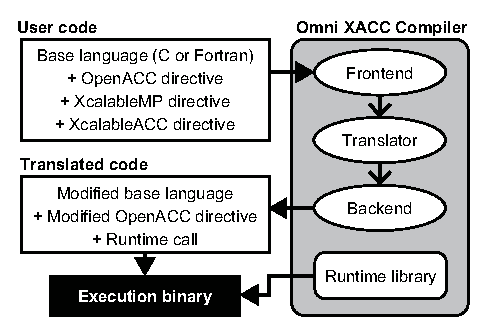
\includegraphics[scale=0.94,clip]{figs/flow2.eps}
\caption{Compile flow of Omni XcalableACC Compiler}
\label{fig:flow}
\end{figure}

Figure \ref{fig:flow} shows the compile flow of Omni XACC Compiler.
First, 
Omni XACC Compiler translates XACC/XMP directives present in the user code into runtime calls. 
Moreover, a part of the base language and OpenACC directives are modified if necessary.
Next, the translated code is compiled by a native compiler to generate an object file.
The native compiler must support OpenACC.
Finally, the object file and the runtime are linked by the native compiler to generate an execution file.
%For details on how Omni Compiler translates the user code, please refer to section V of \cite{nakao2014}.

\begin{figure}[!t]
\begin{center}
\begin{lstlisting}
double a[N];
#pragma xmp template t[N]
#pragma xmp nodes p[4]
#pragma xmp distribute t[block] onto p
#pragma xmp align a[i] with t[i]
...
#pragma acc data copy(a)
{
#pragma xmp loop on t[i]
#pragma acc parallel loop
  for(int i=0;i<N;i++){ 
    a[i] = ... ;
  }
}
\end{lstlisting}
\end{center} 
\caption{Example of XcalableACC code} \label{fig:program}
\end{figure}

\begin{figure}[h]
\begin{center}
\begin{lstlisting}
long long _XACC_start_a  = _XACC_get_array_start_index(_XMP_DESC_a, 0);
long long _XACC_length_a = _XACC_get_array_length(_XMP_DESC_a, 0, N-1);
#pragma acc data copy(_XMP_ADDR_a[_XACC_start_a:_XACC_length_a])
{
  int _XMP_loop_init_i;
  int _XMP_loop_cond_i;
  int _XMP_loop_step_i;
  _XMP_sched_loop_template_BLOCK(0, N, 1, &(_XMP_loop_init_i), &(_XMP_loop_cond_i), &(_XMP_loop_step_i), ...);
#pragma acc parallel loop
  for(int i = _XMP_loop_init_i; i < _XMP_loop_cond_i; i += _XMP_loop_step_i) {
     (*(_XMP_M_GET_ADDR_E_1(_XMP_ADDR_a, i))) = ... ;
  } // end for
} // end acc data
\end{lstlisting}
\end{center} 
\caption{Example of loop statement translation using Omni XcalableACC Compiler} \label{fig:program2}
\end{figure}

%In order to perform parallelization of a loop statement using both XMP and OpenACC, 
Omni XACC Compiler dynamically allocates a reasonable memory for distributed arrays.
According to the OpenACC specification, 
when using dynamic memory allocation, 
the start index and length of the array must be specified in the OpenACC data directive.
Therefore, when using a distributed array in the OpenACC data directive,
Omni XACC Compiler must insert the start index and length of the array.
For example, Omni XACC Compiler translates {\bf \#pragma acc data copy(a)} into {\bf \#pragma acc data copy(a[start:length])} if an array {\bf a} is a distributed array.
The variables {\bf start} and {\bf length} are the start index and length of the distributed array on each node.
Omni XACC Compiler also inserts functions to calculate these values before the OpenACC data directive.
For example, lines 7 to 14 of Figure \ref{fig:program} are translated into  Figure \ref{fig:program2}.
%Omni XACC compiler translates the XMP loop directive and the loop statement.
%Next, Omni XACC compiler inserts the OpenACC {\bf parallel} directive before the loop statement.
%These translations are also shown in lines 5 to 12 of Fig. \ref{fig:program2}.
In line 8 of Fig. \ref{fig:program2}, {\bf \_XMP\_sched\_loop\_template\_BLOCK()} calculates indexes of a loop statement assigned with each node,
and these indexes are used in conditions of the loop statement.
Moreover, 
a distributed array in the loop statement is translated into a pointer calculation.
For example, {\bf \_XMP\_M\_GET\_ADDR\_E\_1()} in Fig. \ref{fig:program2} is an XMP macro to calculate a local index from a global index.
  
In order to transfer data between NVIDIA GPUs across compute nodes,
we implement the following three methods for Omni XACC Compiler.
(1) Using TCA/IB hybrid communication\cite{tca,tca2}.
(2) Using GPUDirect RDMA with CUDA-Aware MPI.
(3) Using MPI and CUDA.
Item (1) performs communication with the smallest latency, but a TCA system is required for the computing environment.
Item (2) is superior in performance to Item (3), but Item (2) also requires specific software and hardware (e.g., MVAPICH2-GDR and Mellanox InfiniBand).
Whereas Items (1) and (2) can realize direct communication between GPUs without the CPU, 
Item (3) copies the data from the accelerator memory to the host memory using CUDA and then transfers the data to other compute nodes using MPI.
Therefore, although Item (3) has the lowest performance, it does not require specific software and hardware.
